%------------------------------------------------------
\subsection{Motivation}
%------------------------------------------------------
\begin{frame} %%Eine Folie
  	\frametitle{Motivation}
  	
\end{frame}
%------------------------------------------------------
\begin{frame} %%Eine Folie
  	\frametitle{Motivation}
  	\begin{center}
  	\small Technologieübersicht verschiedener Tracking-Methoden.
  	\end{center}
%
	\begin{table} [H]
		\begin{center}
			\begin{tabular}{rllll}
				\textbf{Arbeitsweise} & \textbf{Optisch} & \textbf{Magnetisch} & \textbf{Ultraschall} & \textbf{ Funk (UHF)} \\
				\textbf{Genauigkeit} & gut & ausreichend & gut & sehr gut \\
				\textbf{Frequenz} & mittel & hoch & gering & hoch \\
				\textbf{Volumen} & mittel & klein & mittel & groß \\
				\textbf{LOS} & Ja & Ja & Nein & Nein \\
				\textbf{In Vivo} & Nein   & Nein & Nein & Ja \\
%			
			\end{tabular}
		\end{center}
%		\caption[Übersicht Navigationsverfahren]{Grobe Übersicht und Einteilung verschiedener Navigationsverfahren anhand ihres physikalischen Messprinzips.}
		\label{tab:overview_tracking}
	\end{table}  	
\end{frame}
%------------------------------------------------------
\begin{frame} %%Eine Folie
  	\frametitle{Probleme bei Funksystemen}
	\begin{textblock*}{4cm}(8cm,1cm) % {block width} (coords)
		\centering
  		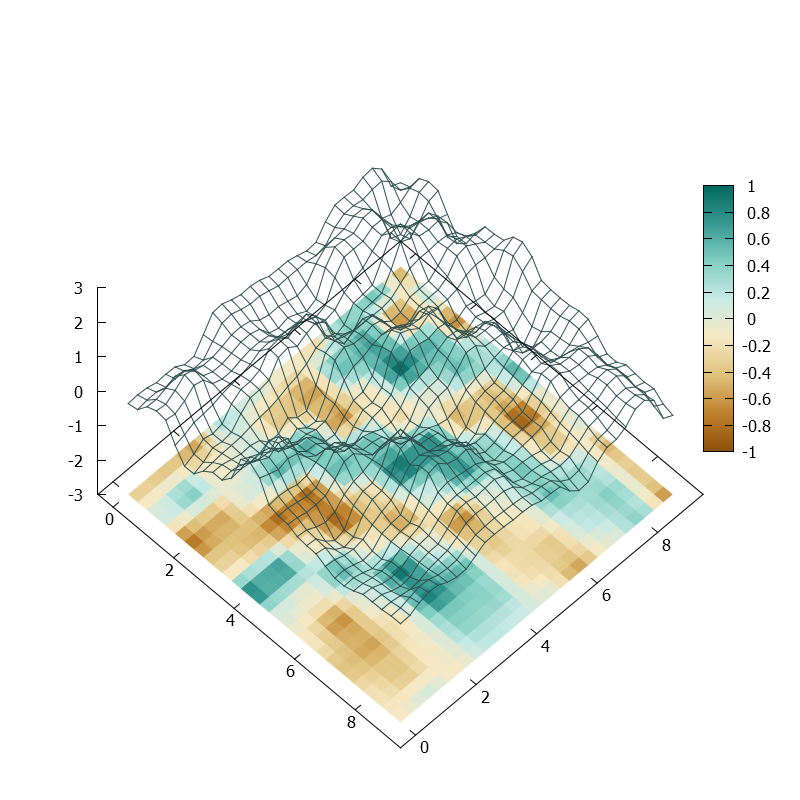
\includegraphics[width=4cm]{../img/Plate0_A1.png}
%  		\footnote{Grafik entnommen aus \url{http://en.wikipedia.org/w/index.php?title=File:Concept_of_directional_optimization_in_CMA-ES_algorithm.png&oldid=532567533}}
  	\end{textblock*}
%  	
	\begin{textblock*}{4cm}(8cm,5cm) % {block width} (coords)
		\centering
  		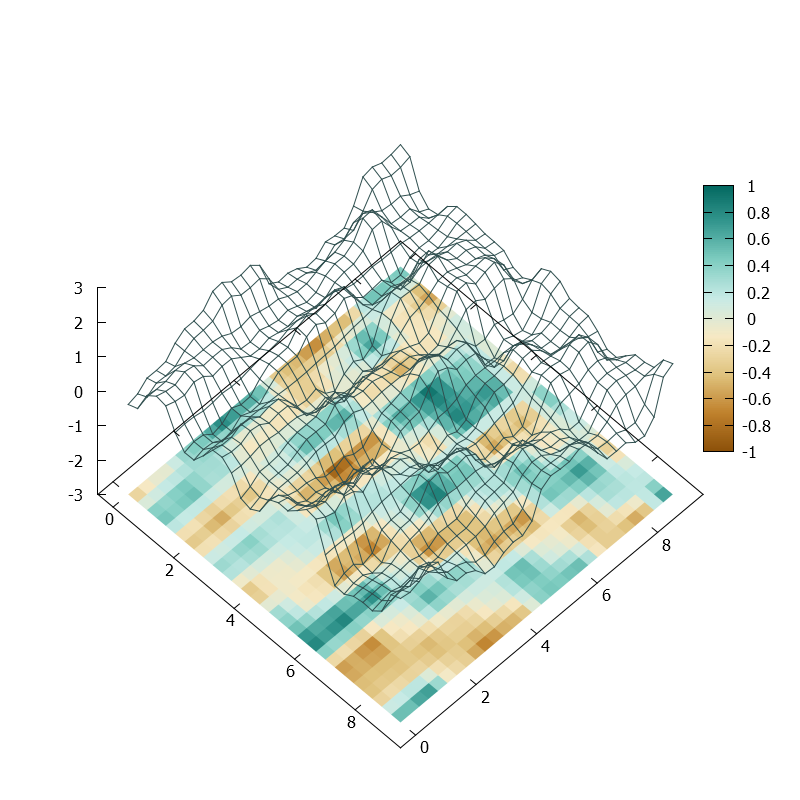
\includegraphics[width=4cm]{../img/Plate0_A4.png}
%  		\footnote{Grafik entnommen aus \url{http://en.wikipedia.org/w/index.php?title=File:Concept_of_directional_optimization_in_CMA-ES_algorithm.png&oldid=532567533}}
  	\end{textblock*}
%  	
	\begin{textblock*}{4cm}(2cm,4cm) % {block width} (coords)
  			\begin{itemize}
  				\item Lücken
  				\item Lesefehler
   				\item Auslöschung
   				\item Reflektionen
  		  	\end{itemize}
  	\end{textblock*}
\end{frame}
%------------------------------------------------------
\subsection{Grundlagen}
%------------------------------------------------------
\begin{frame}{Graphics} 
	\frametitle{Mathematische Grundlagen I }
	\centering
	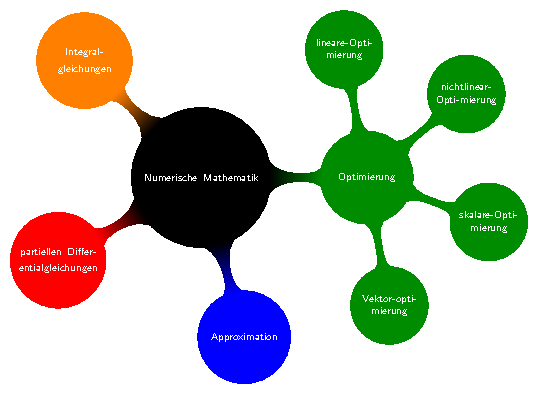
\includegraphics[page=1, width=.6\textwidth]{../img/mindmap.pdf}\\
%--
	\tiny Evolutionäre Verfahren sind Teilgebiet der \textbf{nichtlinearen Optimierung}
\end{frame}
%------------------------------------------------------
\begin{frame}{Graphics} 
  	\frametitle{Mathematische Grundlagen II}
  	\centering
	\includegraphics[page=1, width=.5\textwidth]{../img/FlowChart_EvolutionaryOptimization.pdf}
\end{frame}
%------------------------------------------------------
\begin{frame}{Graphics} 
  	\frametitle{Mathematische Grundlagen III}
%  	
  	\begin{textblock*}{8cm}(4cm,2cm) % {block width} (coords)
  		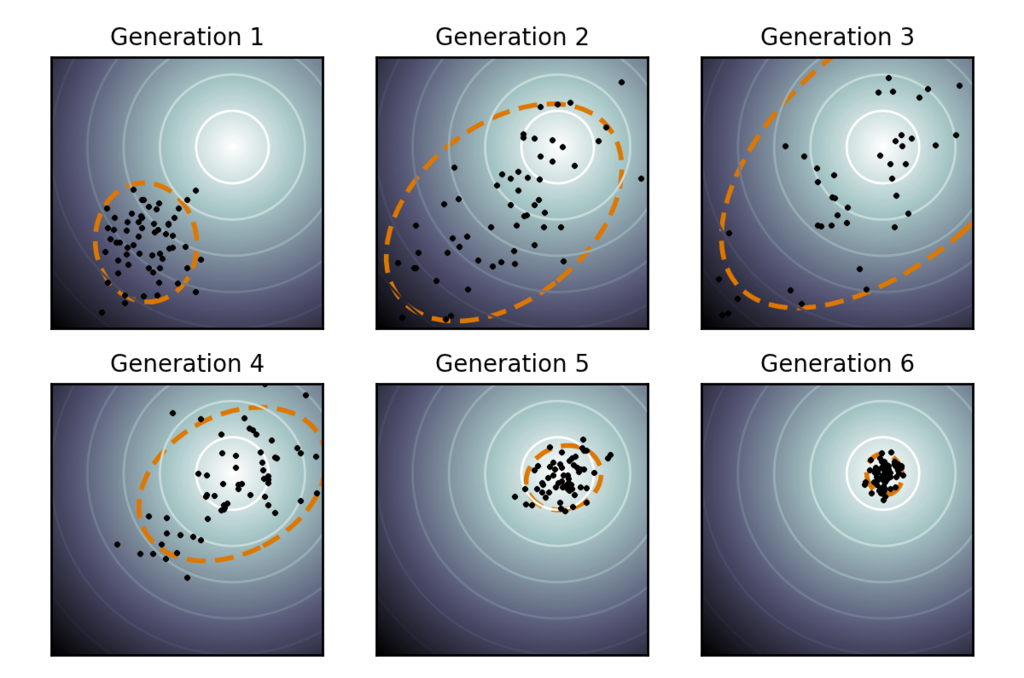
\includegraphics[width=8cm]{../img/Concept_of_directional_optimization_in_CMA-ES_algorithm.png}
  		\footnote{Grafik entnommen aus \url{http://en.wikipedia.org/w/index.php?title=File:Concept_of_directional_optimization_in_CMA-ES_algorithm.png&oldid=532567533}}
  	\end{textblock*}
%  	
\end{frame}
%------------------------------------------------------
\begin{frame} %%Eine Folie
  \frametitle{Beispiele}
%  
  \begin{itemize}
	\item\movie[width=1cm,height=1cm,externalviewer]{Video 1}{../vid/vid1.webm}
	\item\movie[width=1cm,height=1cm,externalviewer]{Video 2}{../vid/vid1.webm}
	\item\movie[width=1cm,height=1cm,externalviewer]{Video 3}{../vid/vid1.webm}
	\item\movie[width=1cm,height=1cm,externalviewer]{Video 4}{../vid/vid1.webm}
  \end{itemize}
%  
\end{frame}
%------------------------------------------------------
\subsection{System der amedo STS}
\begin{frame}
  \frametitle{Messystem}
	\begin{textblock*}{5cm}(7cm,2cm) % {block width} (coords)
  		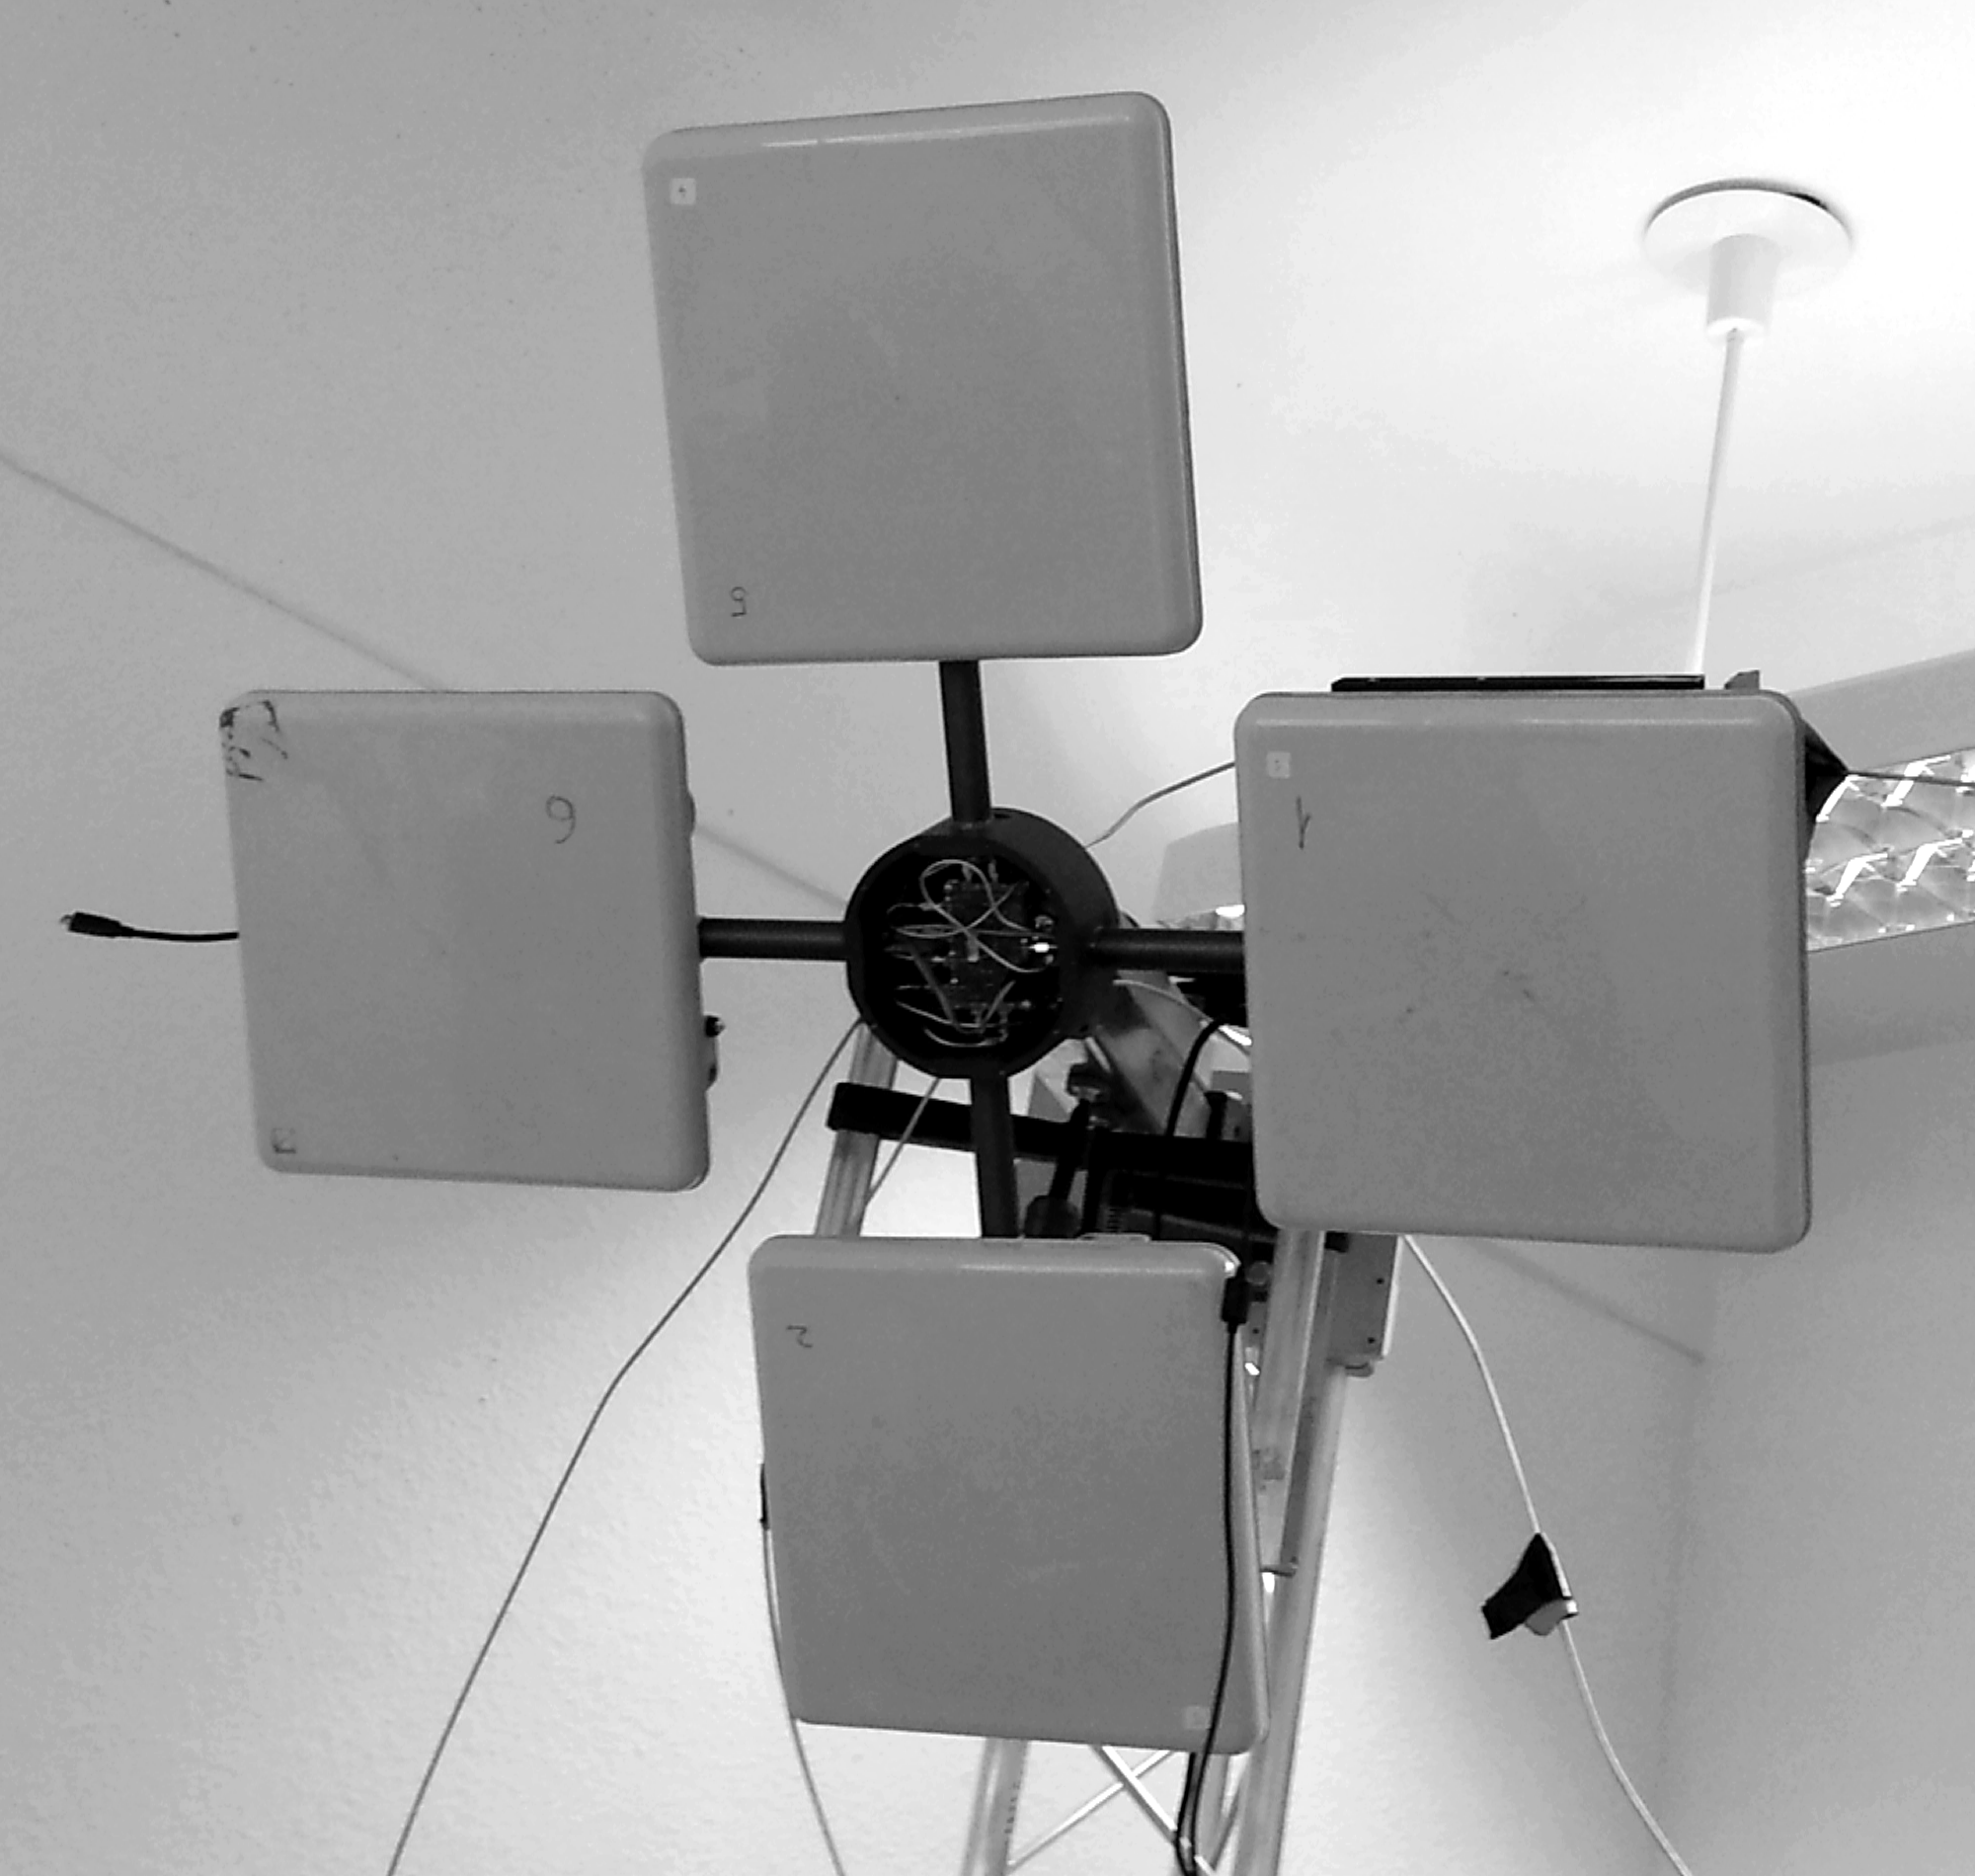
\includegraphics[width=5cm]{../img/4AntennaSetup_small.png}
  	\end{textblock*}
\end{frame}
%------------------------------------------------------
\subsection{System der amedo STS}
\begin{frame}
  \frametitle{Messystem}
	\begin{textblock*}{7cm}(5cm,2cm) % {block width} (coords)
  		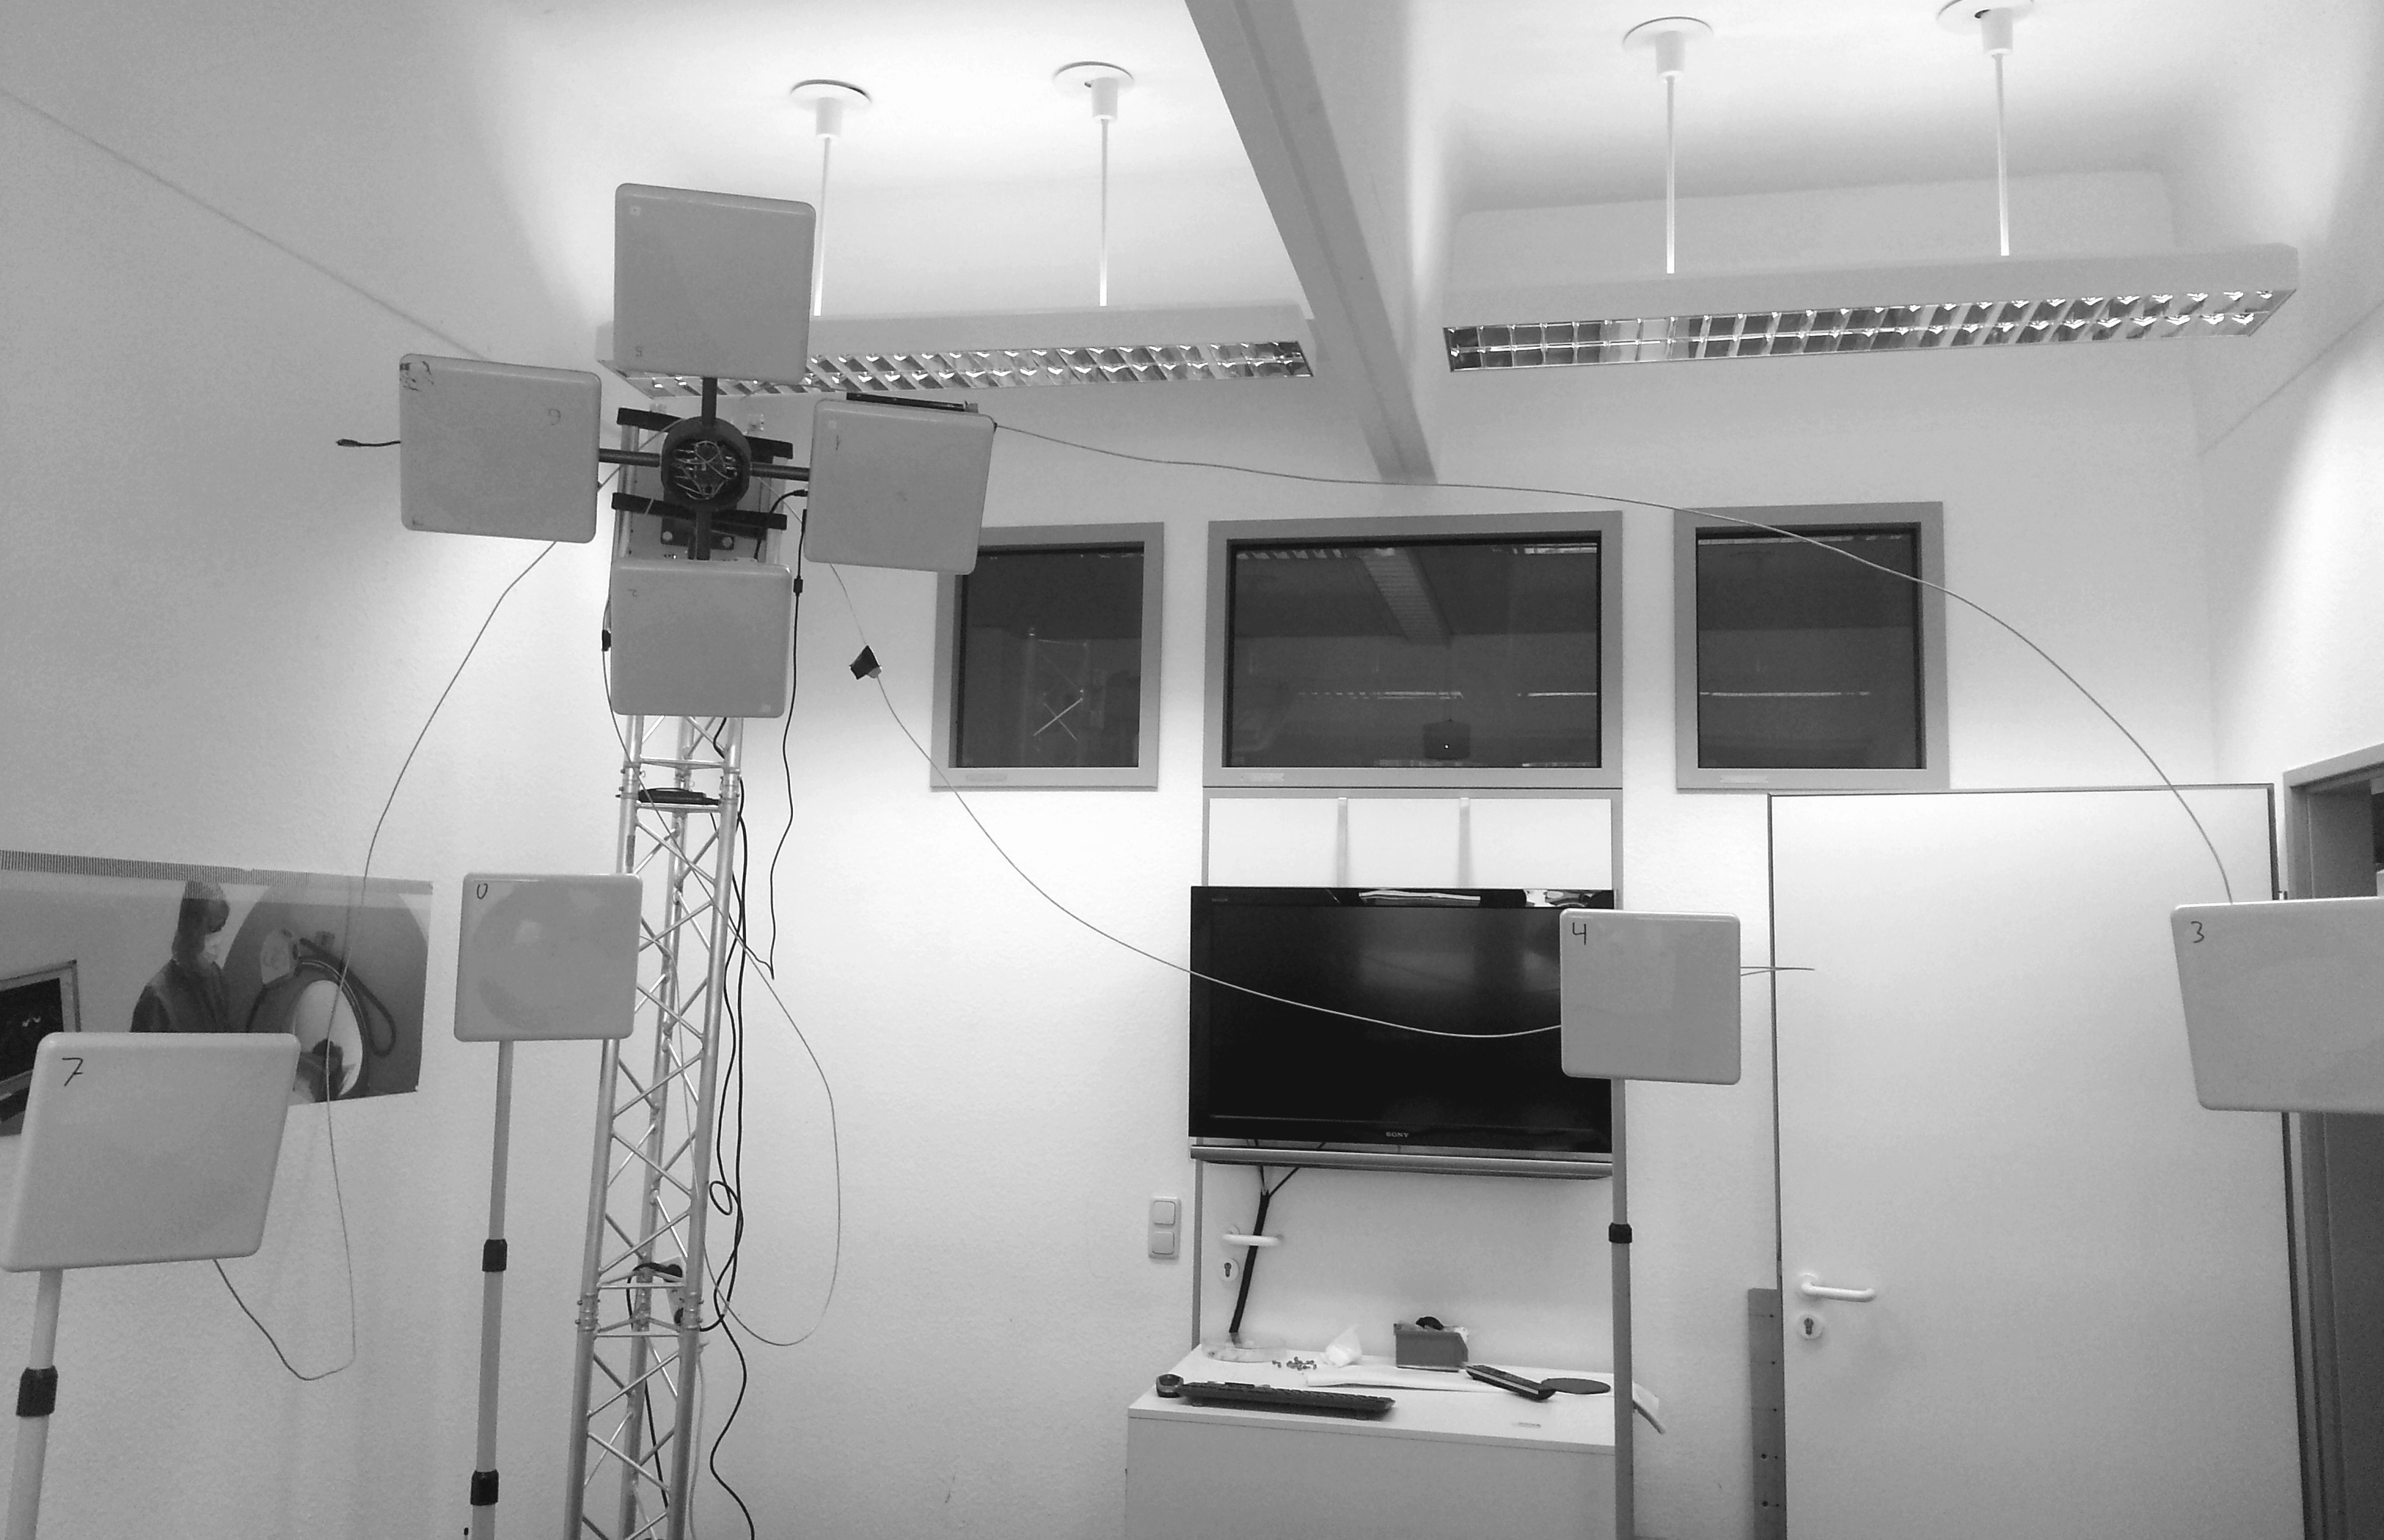
\includegraphics[width=7cm]{../img/RFID-Okto.png}
  	\end{textblock*}
\end{frame}
%------------------------------------------------------
%\subsection{Grundlagen2}
%\begin{frame}
%  \frametitle{Test}
%  \begin{fazit} %%Definition
%    Beschreibung des Problems
%  \end{fazit}
%\end{frame}
